% ============================================================
\chapter{Introduction}
\label{ch:introduction}
% ============================================================

\section{Background}

Urbanisation is reshaping mobility at an unprecedented pace: the United Nations projects that 68\% of the world's population will reside in cities by 2050~\parencite{un2018wup}, intensifying congestion, greenhouse gas emissions, and demand for scalable, on-demand transport.  In New York City alone, taxis and ride-hailing vehicles account for hundreds of millions of trips annually, contributing substantially to urban congestion and vehicular emissions~\parencite{taxinyc_dataset}.  Shared-ride taxi services sit at the intersection of these pressures, capable of door-to-door coverage that mass transit cannot provide, yet environmentally costly when vehicles carry a single passenger.  Realising the potential of shared taxis therefore requires two complementary capabilities: accurate \emph{demand forecasting}, enabling operators to pre-position vehicles and reduce idle mileage, and effective \emph{ride pooling}, so that compatible trips share a vehicle and reduce per-passenger cost and emissions.

Taxi demand forecasting is a spatio-temporal prediction problem of significant practical complexity.  Demand varies sharply by time of day, day of week, weather conditions, and geographic zone, requiring models that can capture both linear trends and non-linear interaction effects simultaneously.  Ensemble methods have shown consistent superiority in tabular prediction tasks~\parencite{breiman2001rf,chen2016xgboost,wolpert1992stacking}, yet no prior study has systematically compared a comprehensive suite of ensemble strategies on the same spatio-temporal demand task with non-parametric statistical validation.  Ride pooling, independently, requires matching algorithms that balance pool rate, per-trip savings, and realistic passenger-acceptance constraints, yet most operational studies either report theoretical upper bounds~\parencite{santi2014quantifying} or fleet-level outcomes without pairwise economic quantification~\parencite{alonso2017demand}.

\section{Research Gap}

Existing literature has explored each capability in isolation.  Demand-forecasting studies, from early data-driven baselines~\parencite{dia2002object} and streaming prediction approaches~\parencite{moreira2013predicting} to deep spatio-temporal networks~\parencite{zhang2017deep,xu2017realtime,kim2020hybrid}, demonstrate steady accuracy gains, yet rarely validate whether observed improvements across model classes are statistically significant.  Ride-pooling analyses such as the shareability network of~\parencite{santi2014quantifying} and the real-time framework of~\parencite{alonso2017demand} report theoretical upper bounds rather than evaluating operational algorithms under realistic passenger-acceptance constraints.  Neither body of work simultaneously quantifies economic and environmental impact at both the trip and city scale.  This thesis addresses all three gaps within a single, reproducible framework evaluated on two years of publicly available New York City Yellow Taxi records.

\section{Objectives and Contributions}

This thesis addresses these gaps through three contributions.

First, a systematic ensemble benchmarking study evaluates fourteen forecasting models on NYC Yellow Taxi data under strictly chronological splits.  A Friedman non-parametric test confirms that observed differences across model classes are statistically significant, with Stacking achieving R\textsuperscript{2}~=~0.9922 and MAPE~=~10.19\%, establishing a strong upper bound for spatio-temporal taxi demand prediction.

Second, a novel LR-LSTM hybrid architecture is proposed in which a Linear Regression stage extracts the deterministic demand trend and an LSTM stage models the non-linear residuals.  An XGBoost-LSTM variant is introduced alongside for comparison, allowing the contribution of each residual-modelling strategy to be isolated and quantified.

Third, a constraint-aware ride pooling algorithm is developed that applies five cascading compatibility filters reflecting realistic passenger-acceptance requirements.  The algorithm achieves a 16.06\% pool rate on 106,055 sampled trips, with projected annual savings of USD~28.7~million and approximately 3{,}370~tonnes of CO\textsubscript{2} for New York City scaled from the sample using the verified 2015 NYC Yellow Taxi annual volume of $\approx$146M trips~\parencite{nyc_opendata_2015}, factor $\approx 1{,}377$, validated through bootstrap resampling with 10,000 iterations.

\section{Thesis Structure}

The remainder of this thesis is organised as follows.  \autoref{ch:related} reviews related work.  \autoref{ch:methods} describes the dataset, preprocessing, spatial clustering, feature engineering, and the ride pooling algorithm.  \autoref{ch:framework} presents the proposed EnsembleNet framework, including individual model architectures, the LR-LSTM hybrid, and the six ensemble strategies.  \autoref{ch:metrics} defines the evaluation metrics.  \autoref{ch:results} reports experimental results and discusses implications, limitations, and future work.  \autoref{ch:conclusion} concludes.

\autoref{fig:intro} presents a high-level overview of the two complementary subsystems that constitute the proposed framework.  The left panel captures the spatial dimension: raw pickup coordinates are partitioned into $K{=}40$ data-driven clusters using MiniBatch KMeans, converting a continuous geographic space into a tractable set of neighbourhood-level demand zones.  Within each zone, demand is aggregated into 10-minute temporal bins, producing a feature matrix that is then enriched with lag features, time-of-day cyclical encodings, weather measurements, and public holiday indicators.  The right panel captures the operational dimension: for any 5-minute window of incoming trips, pairs of rides are evaluated against five cascading filters covering time proximity, origin proximity, destination proximity, route direction alignment, and maximum detour ratio.  Only pairs clearing all five filters receive a weighted compatibility score; a greedy matching pass then assembles the highest-scoring pairs into shared rides.  The two subsystems are designed to operate sequentially in production: demand forecasts inform vehicle pre-positioning, while the pooling algorithm processes the resulting trip requests in real time.  Together they address both the supply-side optimisation problem and the demand-side coordination problem that characterise shared urban mobility.

\begin{figure}[t]
  \centering
  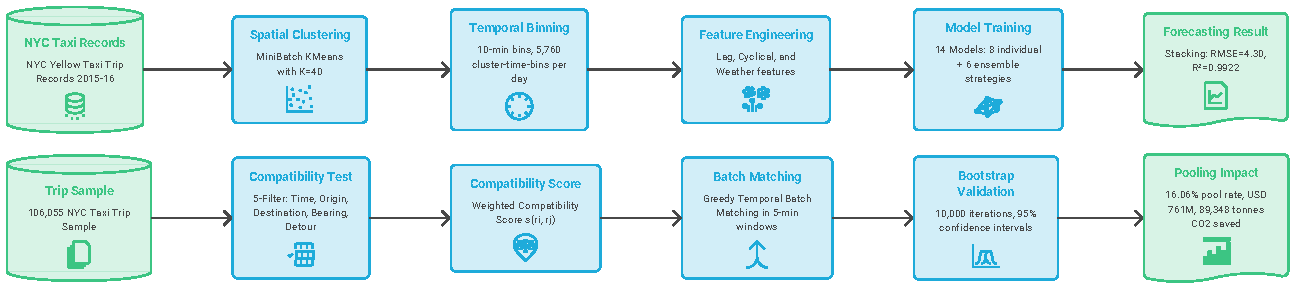
\includegraphics[width=\textwidth, height=0.45\textheight, keepaspectratio]{Figures/Intro.pdf}
  \caption{Overview of the proposed EnsembleNet framework for NYC shared taxi systems. The left panel shows data-driven spatial clustering of pickup locations into $K{=}40$ demand zones and the temporal demand patterns observed within each zone. The right panel depicts the multi-criteria ride pooling matching pipeline, showing how compatible trip pairs are identified and how cost and environmental savings are estimated.}
  \label{fig:intro}
\end{figure}
